\documentclass[10pt, reqno]{amsart}
% \pdfoutput=1



% Packages to open
\usepackage{amsthm, amssymb, amsmath, enumerate, textcomp}
% \usepackage{fullpage}
\usepackage{verbatim}
\usepackage{graphicx, graphics}
\usepackage{algorithm}
\usepackage{longtable}


% Setup TikZ

\usepackage{tikz}
\usetikzlibrary{arrows}
\tikzstyle{block}=[draw opacity=0.7,line width=1.4cm]

% Hopefully dot packages
\usepackage[all,arc,curve,frame,color]{xy}
\usepackage{subfigure}
\usepackage{url}








% \usepackage{setspace}  % Use command \doublespacing or \onehalfspacing

% Standard Theorem Styles
\newtheorem{thm}{Theorem}[section]
\newtheorem{lem}[thm]{Lemma}
\newtheorem{cor}[thm]{Corollary}
\newtheorem*{cor*}{Corollary}
\newtheorem{prop}[thm]{Proposition}
\newtheorem{obs}[thm]{Observation}
\newtheorem{claim}[thm]{Claim}
\newtheorem*{conjecture*}{Conjecture}
\newtheorem{conjecture}[thm]{Conjecture}
\newtheorem*{thm*}{Theorem}
\newtheorem{ps}{Problem Solving Strategy}

\theoremstyle{remark}
\newtheorem*{question*}{Question}
\newtheorem{question}[thm]{Question}
\newtheorem{answer}[thm]{Answer}
\newtheorem*{remark*}{Remark}
\newtheorem{example}[thm]{Example}
\newtheorem*{thinkpair*}{Think/Pair/Share}



\theoremstyle{definition}
\newtheorem{define}[thm]{Definition}
\newtheorem*{define*}{Definition}
\newtheorem{idea}{Idea}
\newtheorem{problem}{Problem}
\newtheorem{exercise}[thm]{Exercise}
\newtheorem*{problem*}{Problem}
\newtheorem*{sol*}{Solution}


\numberwithin{equation}{section}  % number equations by section

% Standard shortcuts
\newcommand{\LL}{\mathcal{L}}     % Fancy script L
\newcommand{\MM}{\mathcal{M}}  % Fancy script M
\newcommand{\OO}{\mathcal{O}}    % Fancy script O
\newcommand{\FF}{\mathbb{F}}      % Finite field
\newcommand{\ZZ}{\mathbb{Z}}     % Integers
\newcommand{\RR}{\mathbb{R}}     % Reals
\newcommand{\PP}{\mathbb{P}}      % Projective space
\newcommand{\Aff}{\mathbb{A}}      % Affine space
\newcommand{\XX}{\mathcal{X}}      % Model of a variety - script X
\newcommand{\QQ}{\mathbb{Q}}      %Rationals
\newcommand{\CC}{\mathbb{C}}      % Complex Numbers
\newcommand{\mm}{\mathfrak{m}}   % maximal ideal
\newcommand{\pp}{\mathfrak{p}}   % prime ideal
\newcommand{\qq}{\mathfrak{q}}  % another prime ideal
\newcommand{\Gm}{\mathbb{G}_m}  % blackboard bold G for the multiplicative group
\newcommand{\hh}{\mathfrak{h}}  % Upper half plane
\newcommand{\tab}{\hspace{.4cm}} % Tab 



 % Color comments!
\usepackage{xcolor}
% Color comments



%Notes to ourselves
\newcommand{\fellow}[1]{{\color{magenta} \sf $\clubsuit\clubsuit\clubsuit$ Fellow: [#1]}}
\newcommand{\michelle}[1]{{\color{blue} \sf $\clubsuit\clubsuit\clubsuit$ Michelle: [#1]}}


% Some regularly used operator shortcuts
\newcommand{\Hom}{\operatorname{Hom}}
\newcommand{\im}{\operatorname{im}} % Image
\newcommand{\coker}{\operatorname{coker}}  % Cokernel
\newcommand{\Sym}{\operatorname{Sym}}      % Symmetric product
\newcommand{\Spec}{\operatorname{Spec}}
\newcommand{\ord}{\operatorname{ord}}
\newcommand{\Div}{\operatorname{div}}    % Divisor of a rational function
\newcommand{\Gal}{\operatorname{Gal}}  % Galois group
\newcommand{\Gauss}{\operatorname{Gauss}}  % Used for the Gauss point
\newcommand{\supp}{\operatorname{supp}}   % Support
\newcommand{\Pic}{\operatorname{Pic}}        % Picard Groups
\newcommand{\Jac}{\operatorname{Jac}}       % Jacobian Variety
\newcommand{\mult}{\operatorname{mult}}  % multiplicity
\newcommand{\pr}{\operatorname{pr}}     % projection
\newcommand{\sep}[1]{{#1}^{\operatorname{s}}}    % separable closure
\newcommand{\Spf}{\operatorname{Spf}}    % formal spectrum
\newcommand{\Frac}{\operatorname{Frac}}    % Fraction field
\newcommand{\chern}[1]{c_1\left(#1\right)}   % First Chern class
\newcommand{\codim}{\operatorname{codim}}  % codimension
\newcommand{\dist}{\operatorname{dist}}   % distance
\newcommand{\an}[1]{\operatorname{an}}  % analytic space notation
\newcommand{\Aut}{\operatorname{Aut}}   % Automorphism group
\newcommand{\Rat}{\operatorname{Rat}}    % space of rational maps
\newcommand{\PGL}{\operatorname{PGL}}
\newcommand{\PSL}{\operatorname{PSL}}
\newcommand{\alg}[1]{{\overline{#1}}}
\newcommand{\GG}{\mathbb{G}}


% Miscellaneous notational shortcuts
\newcommand{\leftexp}[2]{{\vphantom{#2}}^{#1}{#2}}   % Superscript on the left
\newcommand{\simarrow}{\stackrel{\sim}{\rightarrow}}    % Isomorphic mapping
\newcommand{\ip}[2]{\left\langle #1,#2 \right\rangle} %inner product
\newcommand{\into}{\hookrightarrow}     % Inclusion arrow
\newcommand{\dint}{\int \!\!\! \int}   % double integral
\newcommand{\tth}{^{\operatorname{th}}}
\newcommand{\Berk}{\mathbf{P}}  % Berkovich Projective Space

\newcommand{\Manoa}{M\=anoa}
\newcommand{\Hawaii}{Hawai\kern.05em`\kern.05em\relax i}


% Document Specific Declarations
\newcommand{\id}{\mathrm{id}}
\newcommand{\oo}{\mathfrak{o}}
\DeclareMathOperator{\Per}{Per}
\DeclareMathOperator{\PrePer}{PrePer}
\DeclareMathOperator{\Twist}{Twist}
\DeclareMathOperator{\Ker}{Ker}


%%%%%%%%%%%%%%

\title{Chapter 2: Place Value}





%%%%%%%%%%%%%%


\begin{document}


\maketitle

\fellow{Formatting: can we put things marked ``Problem'' in a box (maybe with some color?) to set it apart?  Same with the Think/Pair/Share (different color?) and Solutions.}

\section{Dots and Boxes}

Here are some dots; in fact there's nine of them.

\begin{center}

\includegraphics[height=3cm]{dots1}
\end{center}

Here are some boxes:

\begin{center}
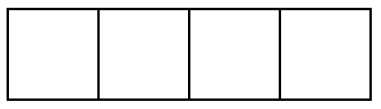
\includegraphics[height=1.5cm]{boxes1}
\end{center}

We're going to a play a game in which boxes explode dots and move them around.  Here's our first rule:

\fellow{Have the rules set off in a box somehow?}

\begin{quote}
{\bf The $1 \leftarrow 2$ Rule:\\
Whenever there are two dots in single box, they ``explode,'' disappear, and become one dot in the box to the left.}
\end{quote}

\begin{example}[Nine dots in the $1 \leftarrow 2$ system]
We start by placing nine dots in the rightmost box.

\begin{center}
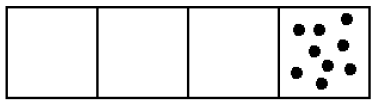
\includegraphics[height=1.5cm]{9dots1}
\end{center}
Two dots in that box explode and become one dot in the box to the left.
\begin{center}
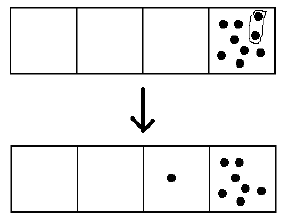
\includegraphics[height=4.5cm]{9dots2}
\end{center}
Since there are more than two dots in the rightmost box, it can happen again.
\begin{center}
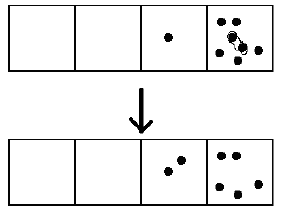
\includegraphics[height=4.5cm]{9dots3}
\end{center}
And again!
\begin{center}
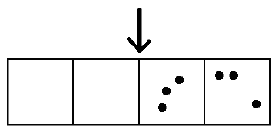
\includegraphics[height=3cm]{9dots4}
\end{center}
Hey, now we have more than two dots in the second box, so those can explode and move!
\begin{center}
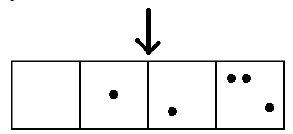
\includegraphics[height=3cm]{9dots5}
\end{center}
And the rightmost box still has more than two dots.
\begin{center}
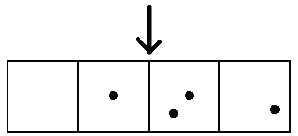
\includegraphics[height=3cm]{9dots6}
\end{center}
Keep going, until no box has two dots.
\begin{center}
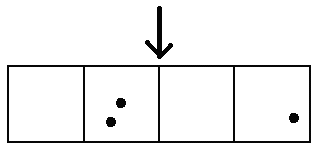
\includegraphics[height=3cm]{9dots7}

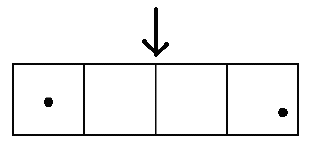
\includegraphics[height=3cm]{9dots8}
\end{center}
After all this, reading from left to right we are left with one dot, followed by zero
dots, zero dots, and one final dot. 

\begin{center}
The $1 \leftarrow 2$ code for nine dots is: \qquad 1001
\end{center}
\end{example}


\subsection*{On Your Own}
Here's a diagram showing what happens for seven dots in a $1 \leftarrow 2$ box.  Trace through the diagram, and circle the pairs of dots that ``exploded'' at each step.

\begin{center}
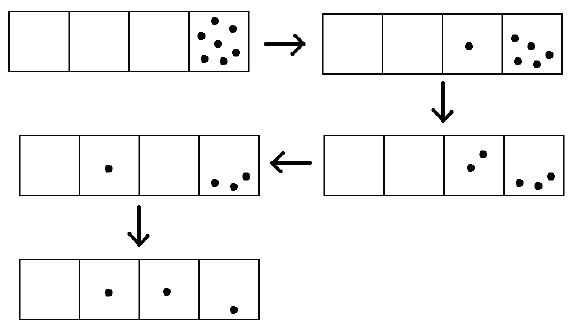
\includegraphics[height=7cm]{7dots}
\end{center}

\begin{center}
The $1 \leftarrow 2$ code for seven dots is: \qquad 111
\end{center}



\begin{problem}
Note: In solving this problem, you don't need to draw on paper; that can get tedious!  Maybe you could use buttons or pennies for dots and do this by hand. What could you use for the boxes?

\begin{enumerate}[(a)]

\item
Draw 10 dots in the right-most box and perform the explosions. What
is the $1 \leftarrow 2$ code for  ten dots?
\item
Find the $1 \leftarrow 2$ code for thirteen dots.
\item
Find the $1 \leftarrow 2$ code for six dots.
\item
What number of dots has $1 \leftarrow 2$ code 101?
\end{enumerate}
\end{problem}

\begin{thinkpair*}
After you worked on the problem, compare your answer with a partner.  Did you both get the same code?  Did you have the same process?
\end{thinkpair*}



\section{Other Rules}
Let's play the dots and boxes game, but change the rule.

\fellow{Have the rules set off in a box somehow?}

\begin{quote}
{\bf The $1 \leftarrow 3$ Rule:\\
Whenever there are three dots in single box, they ``explode,'' disappear, and become one dot in the box to the left.}
\end{quote}

\begin{example}[Fifteen dots in the $1 \leftarrow 3$ system]
Here's what happens with fifteen dots:
\begin{center}
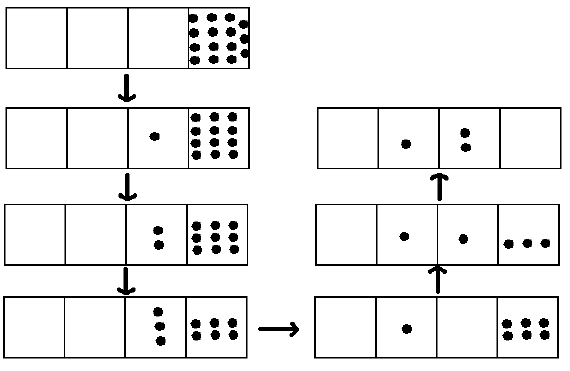
\includegraphics[height=8cm]{15dots}
\end{center}

\begin{center}
The $1 \leftarrow 3$ code for seven dots is: \qquad 120
\end{center}


\end{example}

\begin{problem}\ 

\begin{enumerate}[(a)]
\item
Show that the $1 \leftarrow 3$ code for twenty dots is 202.
\item
Show that the $1 \leftarrow 3$ code for four dots is 11.
\item
What is the  $1 \leftarrow 3$ code for thirteen dots?
\item
What is the  $1 \leftarrow 3$ code for twenty-five dots?
\item
What number of dots has  $1 \leftarrow 3$ code 1022? 
\item
Is it possible for a collection of dots to have  $1 \leftarrow 3$ code 2031?  Explain your answer.

\end{enumerate}
\end{problem}


\begin{problem}\ 

\begin{enumerate}[(a)]
\item
Describe how the $1 \leftarrow 4$ rule would work.
\item
What is the $1 \leftarrow 4$ code for the number thirteen?
\end{enumerate}
\end{problem}

\begin{problem}\ 

\begin{enumerate}[(a)]
\item
What is the $1 \leftarrow 5$ code for the number thirteen?
\item
What is the $1 \leftarrow 5$ code for the number five?
\end{enumerate}
\end{problem}


\begin{problem}\ 

\begin{enumerate}[(a)]
\item
What is the $1 \leftarrow 9$ code for the number thirteen?
\item
What is the $1 \leftarrow 9$ code for the number thirty?
\end{enumerate}
\end{problem}


\begin{problem}\label{prob:Base10}\ 

\begin{enumerate}[(a)]
\item
What is the $1 \leftarrow 10$ code for the number thirteen?
\item
What is the $1 \leftarrow 10$ code for the number thirty-seven?
\item
What is the $1 \leftarrow 10$ code for the number two hundred thirty-eight?
\item
What is the $1 \leftarrow 10$ code for the number five thousand eight hundred and thirty-three?
\end{enumerate}
\end{problem}

\begin{thinkpair*}
After you have worked on the problems on your own, compare your ideas with a partner.  Can you describe what's going on in Problem~\ref{prob:Base10} and why?
\end{thinkpair*}



\section{Binary Numbers}\label{sec:Binary}
Let's go back to the $1 \leftarrow 2$ rule for a moment:
\begin{quote}
{\bf The $1 \leftarrow 2$ Rule:\\
Whenever there are two dots in single box, they ``explode,'' disappear, and become one dot in the box to the left.}
\end{quote}

Two dots in the right-most box is worth one dot in the next box to the left.
\begin{center}
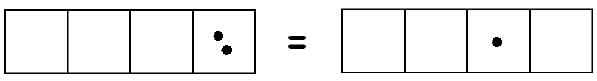
\includegraphics[height=1.5cm]{binary1}
\end{center}
If each of the original dots is worth ``one,'' then the single dot on the left must be worth two.
\begin{center}
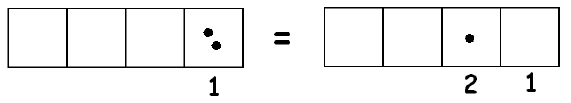
\includegraphics[height=2cm]{binary2}
\end{center}
But we also have two dots in the box of value 2 is worth 1 dot in the box just to the left\dots
\begin{center}
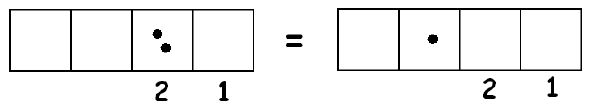
\includegraphics[height=2cm]{binary3}
\end{center}
So that next box must be worth two 2s, which is four!
\begin{center}
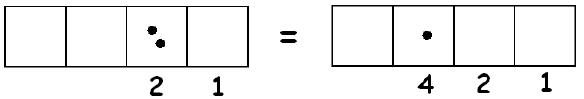
\includegraphics[height=2cm]{binary4}
\end{center}
And two of these fours make eight.
\begin{center}
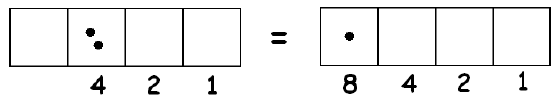
\includegraphics[height=2.1cm]{binary5}
\end{center}


\begin{example}
We said earlier that the $1 \leftarrow 2$ code for nine dots was 1001. Let�s check:
\begin{center}
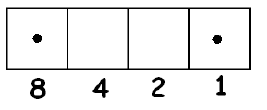
\includegraphics[height=2.1cm]{9inbinary}
\end{center}
\[
8 + 1 = 9,  \text{ so this works!}
\]
We also said that thirteen has $1 \leftarrow 2$ code 1101. This is correct.
\begin{center}
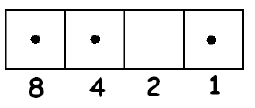
\includegraphics[height=2.1cm]{13inbinary}
\end{center}
\[
\text{Yep!} \quad 8+4+1 = 13.
\]

\end{example}


\begin{problem}\label{prob:BinaryStart}\ 

\begin{enumerate}[(a)]
\item
If there were a box to the left of the 8 box, what would the value of that box be?
\item
What would be the value of a box \emph{two} spots to the left of the 8 box?  Three spots to the left?
\item
What number has $1 \leftarrow 2$ code 100101?
\item
What is the $1 \leftarrow 2$ code for the number two hundred? 
\end{enumerate}
\end{problem}



\begin{define}
Numbers written in the $1 \leftarrow 2$ code are called \emph{binary numbers} or \emph{base two} numbers.  (The prefix ``bi'' means ``two.'')  From now on, when we want to indicate that a number is written in base two, we will write a subscript ``two'' on the number.  So $1001_{\text{two}}$ means ``the number of dots that has $1\leftarrow 2$ code 1001,'' which we already saw was nine.

\end{define}


Important! When we read $1001_{\text{two}}$ we say ``one zero zero one base two.''  We don't say ``one thousand and one,'' because ``thousand'' is not a binary number.



\begin{thinkpair*}
Compare you work on problem~\ref{prob:BinaryStart} with a partner.  
\begin{itemize}
\item
Your first goal: come up with a \emph{general method} to find the number of dots represented by any binary number.  Clearly describe your method.  Test your method out on these numbers, and check your work by actually ``unexploding'' the dots.
\[
1_{\text{two}}
\qquad
101_{\text{two}}
\qquad
1011_{\text{two}}
\qquad
1111_{\text{two}}
\qquad
1101101_{\text{two}}
\]

\item
Explain why binary numbers only contain the digits 0 and 1.

\item
Here is a new (harder) goal: come up with a \emph{general method} to find the binary number related to any number of dots \emph{without actually going through the ``exploding dot'' process}.  Clearly describe your method.  Test your method out on these numbers, and find a way to check your work.
\[
 \text{two dots } = ???_{\text{two}}
\qquad\quad
 \text{seventeen dots } = ???_{\text{two}}
\qquad\quad
 \text{sixty-four dots } = ???_{\text{two}}
 \]
 \[
 \text{sixty-three dots } = ???_{\text{two}}
\qquad\qquad
 \text{one thousand dots } = ???_{\text{two}}
\]
\end{itemize}

\end{thinkpair*}

\subsection{Binary Numbers and Computers}
\fellow{Can you write a \emph{short} description of the use of binary numbers in computers?  Just a paragraph or two getting across the main ideas.}





\section{Other Bases}
In the $1 \leftarrow 3$ system, three dots in one box is worth one dot
in the box one spot to the left. This gives a new picture:
\begin{center}
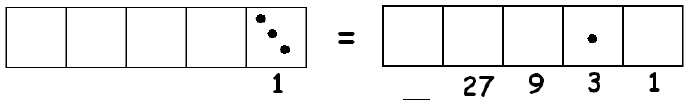
\includegraphics[height=2.1cm]{base3_1}
\end{center}
Each dot in the second box from the left is worth three ones.  Each dot in the third box is worth three 3s, which is nine, and so on.

\begin{example}
We said that the $1\leftarrow 3$ code for fifteen is 120. We see that this is correct
because
\begin{center}
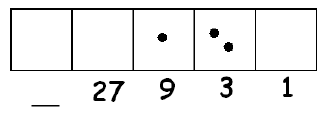
\includegraphics[height=2.5cm]{15base3}
\end{center}
\[
9 + 2\cdot 3 = 9+6 = 15.
\]
\end{example}


\begin{problem}\label{prob:Base3Start}
Answer these questions about the $1 \leftarrow 3$ system.

\begin{enumerate}[(a)]
\item
What label should go on the box to the left of the 27 box?
\item
What would be the value of a box \emph{two} spots to the left of the 27 box?
\item
What number has $1 \leftarrow 3$ code 21002?
\item
What is the $1 \leftarrow 3$ code for the number two hundred?  
\end{enumerate}
\end{problem}

\begin{problem}
In the $1 \leftarrow 4$ system, four dots in one box are worth one dot in the box one place
to the left. 
\begin{enumerate}[(a)]
\item
What is the value of each box?
\begin{center}
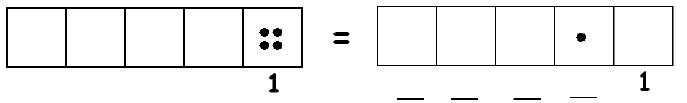
\includegraphics[height=2cm]{base4system}
\end{center}

\item
What is the $1 \leftarrow 4$ code for twenty-nine?

\item
What number has $1 \leftarrow 4$ code 132?
\end{enumerate}

\end{problem}


\begin{problem}
In the $1 \leftarrow 10$ system, ten dots in one box are worth one dot in the box one place
to the left. 
\begin{enumerate}[(a)]
\item
What is the value of each box?
\begin{center}
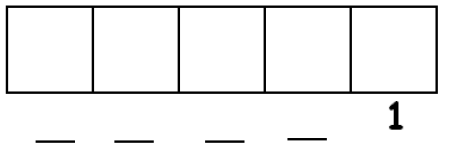
\includegraphics[height=2cm]{base10system}
\end{center}

\item
What is the $1 \leftarrow 10$ code for eight thousand four hundred and twenty-two?

\item
What number has $1 \leftarrow 10$ code 95753?

\item
When we write the number 7842 the ``7'' is represents what quantity? The ``4'' is
four groups of what value? The ``8'' is eight groups of what value? The ``2'' is two
groups of what value?

\item
Why do human beings like the $1\leftarrow 10$ system for writing numbers? 
\end{enumerate}

\end{problem}


\begin{define}
Numbers written in the  $1 \leftarrow 3$ system are called \emph{base three numbers}.  Numbers written in the $1 \leftarrow 4$ system are called \emph{base four numbers}.  Numbers written in the $1 \leftarrow 10$ system are called \emph{base ten numbers}.  In general, numbers written in the $1 \leftarrow b$ system are called \emph{base $b$ numbers.}

\end{define}

In a base $b$ number system, each place represents a \emph{power of $b$}, which means $b^k$ for some positive number $k$.  Remember this means $b$ multiplied by itself $k$ times:
\[
b^k = \underbrace{b \cdot b \cdots b}_{k \text{ times}}.
\]
\begin{itemize}
\item
The right-most place is the \emph{units} or \emph{ones} place.  (Why is this a \emph{power of $b$?})
\item
The second spot is the ``$b$'' place.  (In base 10, it's the tens place.)
\item
The third spot is the ``$b^2$'' place.  (In base 10, that's the hundreds place, and $100 = 10^2$.)
\item
The fourth spot is the ``$b^3$'' place.  (In base 10, that's the thousands place, and $1000 = 10^3$.)
\item
And so on\dots the $n^\text{th}$ spot is the $b^{n-1}$ place.
\end{itemize}

{\bf Notation:}
Whenever we're dealing with numbers written in different bases, we use a subscript to indicate the base so that there can be no confusion.  So $102_\text{three}$ is a base three number,  $222_\text{four}$ is a base four number, and $54321_\text{ten}$ is a base ten number.  If the base is not written, we assume the number is written in base ten. 



\begin{thinkpair*}\ 
\begin{enumerate}[(a)]
\item
Find the number of dots represented by:
\[
102_\text{three}, 
\quad 222_\text{four}, 
\quad 
54321_\text{ten}.
\]
\item
Represent nine dots in each base: 
\begin{center}
 three, four, five, six, seven, eight, nine, and ten.
\end{center}
\item
Which digits are used in the base two system?  The base three system?  The base four system?  The base five system?  The base six system?  The base ten system?
\item
What does the \emph{base} tell you about the number system?  (Think of as many answers as you can!)
\end{enumerate}
\end{thinkpair*}


\subsection{Base $b$ to Base Ten}
In Section \ref{sec:Binary}, you were asked to come up with \emph{general methods} to translate numbers from base two (binary) to  base ten (our standard system).  We're now going to describe some general methods for converting from base $b$  to base ten, where $b$ can represent any whole number bigger than one.

If the base is $b$, that means we're in a $1 \leftarrow b$ system.  A dot in the right-most box is worth 1.  A dot in the second box is worth $b$.  A dot in the third box is worth $b \times b = b^2$, and so on.

\fellow{Can you make a picture of base $b$ boxes with the appropriate labels, say up to  $b^4$?}

So, for example, the number $10123_b$ represents
\[
1\cdot b^4  + 0 \cdot b^3 +  1 \cdot b^2  + 2\cdot b + 3\cdot 1 \text{ dots,}
\]
because we imagine three dots in the right-most box (each worth one), two dots in the second box (each representing $b$ dots), one dot in the third box (representing $b^2$ dots), and so on.  That means we can just do a short calculation to find the total number of dots, without going through all the trouble of drawing the picture and  ``unexploding'' the dots.

\begin{example}
Consider the number $123_\text{five}$.  This represents
\[
 1 \cdot 5^2  + 2 \cdot 5 + 3 = 25 + 10 + 3 = 38 \text{ dots.}
\]
On the other hand,  the number $123_\text{seven}$ represents
\[
 1 \cdot 7^2  + 2 \cdot 7 + 3 = 49 + 14 + 3 = 66 \text{ dots.}
\]

\end{example}


\begin{thinkpair*}\ 
\begin{itemize}
\item
Convert each number to base ten.  Compare your answers with a partner to be sure you agree.

\[
18_\text{nine},
\qquad
547_\text{eight},
\qquad
3033_\text{five},
\qquad
11011_\text{three}.
\]

\item
Which number represents a greater amount of total dots:  
\[
23,455,443_\text{six} \quad \text{ or } \quad 23,455,443_\text{eight}?
\]
  Justify your answer.
\end{itemize}
\end{thinkpair*}


\subsection{Base Ten  to Base $b$}
In Section \ref{sec:Binary}, you were also asked to come up with \emph{general methods} to translate numbers from base ten to  base two.  We're now going to describe some general methods for converting from base ten to  base $b$, where $b$ can represent any whole number bigger than one.

We'll work out an example, and then describe the general method.  

\begin{example}
To convert $321$ to a base five number  (without actually going through the tedious process of exploding $321$ dots in groups of five):


Find the largest power of five that is smaller than 321.  We'll just list powers of five:
\[
5^1 = 5, \quad 5^2 = 25, \quad 5^3 = 125, \quad 5^4 = 625.
\]
So we know that the left-most box we'll use is the $5^3$ box.  
\fellow{add a picture of the appropriately labeled boxes for base 5, up to $5^3$?}

How many dots will be in that left-most box?  That's the same as asking how many 125s are in 321.  Since
\[
2\cdot 125 = 250 \quad \text{ and } \quad 3 \cdot 125 = 375,
\]
we have two dots in the $5^3$ box, representing a total of $250$ dots, but rather than drawing dots we'll start writing the digits to represent them.

\fellow{picture of the base 5 boxes with a ``2'' in  the $5^3$ box?}

How many dots are left unaccounted for?  $321 - 250 = 71$ dots are left.

Now just repeat the process: We can put a ``2'' in the $5^2$ box, and that takes care of $50$ dots.  So so far we have two in the $5^3$ box and two  in the $5^2$ box, so that's a total of 
\[
2\cdot 125 + 2\cdot 25 = 300 \text{ dots}.
\]

\fellow{picture of the base 5 boxes with 2 in $5^3$ box and 2 in the $5^2$ box?}

We have $21$ dots left to account for.  The biggest power of $5$ that's less than 21 is just $5$.  So we can put a ``4'' in the $5$ box, and we have one  left over in the one box.

\fellow{picture of the base 5 boxes with 2 in $5^3$ box and 2 in the $5^2$ box 4 in the $5$ box and 1 in the $1$ box?}

\[
2\cdot 125 + 2\cdot 25 + 4\cdot 5 + 1= 250 + 50 + 20 + 1 =  321 \text{ dots}.
\]
\[
\text{So } 321 = 2241_\text{five}.
\]
\end{example}

The general algorithm to convert from base ten to base $b$:
\begin{enumerate}
\item
Start with your base ten number $n$.  Find the largest \emph{power of $b$} that's less than your number $n$, say that power is $b^k$.  
\item
Figure out how many dots can go in the $b^k$ box without going over the number $n$.  Say that number is $a$.  Put the digit $a$ in the $b^k$ box, and then subtract $n - a\cdot b^k$ to figure out how many dots are left.
\item
If your number is now zero, you accounted for all the dots.  Put zeros in any boxes that remain, and you have the number.  Otherwise, start over at step (1) with the number of dots you have left.

\end{enumerate}

The method seems a little tricky to describe in complete generality.  It's probably better to try a few examples on your own to get the hang of it.

\begin{thinkpair*}
Use the method above to convert $99_\text{ten}$ to base three, to base four, and to base five.
\end{thinkpair*}

The first method we described fills in the boxes from left to right.  Here's another method to convert base ten numbers to another base, and this method fills in the digits from right to left.  Again, we'll start with an example and then describe the general method:

\begin{example}
To convert $712$ to a base seven number:

Divide $712$ by seven and find the quotient and remainder:
\[
712 \div 7 = 101 \text{ R}5.
\]
Put the remainder in the ones place: 
\[
712 = \underline{???}5_\text{seven}.
\]

Now take the quotient and divide by seven to find the quotient and remainder:
\[
101 \div 7 = 14 \text{ R}3.
\]
Put the remainder in the sevens place: 
\[
712 = \underline{???}35_\text{seven}.
\]

Take the previous quotient and divide by seven again:
\[
14 \div 7 = 2 \text{ R}0.
\]
Put the remainder in the $7^2$ place: 
\[
712 = \underline{???}035_\text{seven}.
\]

Since the quotient that's left is less than seven, it goes in the $7^3$ place, and we're done.
\[
712 = 2035_\text{seven}.
\]

Of course, we can (and should!) check our calculation by converting the answer back to base ten:
\[
2035_\text{seven} = 2\cdot 7^3 + 0 \cdot 7^2 + 3 \cdot 7 + 5 
= 686 + 0 + 21 + 5 = 712_\text{ten}.
\]

\end{example}

So here's a second general method for converting base ten numbers to an arbitrary base $b$:
\begin{enumerate}
\item
Divide the base ten number by $b$ to get a quotient and a remainder. 
\item
Put the remainder in the right-most space in the base $b$ number.
\item
If the quotient is less than $b$, it goes in the space one spot to the left.  Otherwise, go back to step (1) and repeat it with the quotient, filling in the remainders from right to left in the base $b$ number.
\end{enumerate}

We can use the dots and boxes system to explain why this method of quotients and remainders works.   It's not just a ``trick!''  We'll stick with the example of converting $712$ to base seven, so we have something specific to talk about.


\begin{itemize}
\item
We imagine 712 dots in the right-most box, since that represents 712 dots total.  Since we're converting to base seven, we're in the $1 \leftarrow 7$ system.
\fellow{picture of the base seven boxes up to $7^3$ with just the number 721 in the right-most box.}


\item
Groups of seven dots will explode, and each group of seven becomes one dot in the next box.  How many groups of seven dots are there?  Well, there are 101 groups of seven, with 5 dots left over out of a group.  That's what we figured out with the calculation
\[
712 \div 7 = 101 \text{ R}5.
\]

\item
Imagine we explode all the groups of seven that we can make in the right-most box before we move on.  Then we would have
 5 dots left in that first  box, and 101 dots in the second box.  
 
 \fellow{picture of the base seven boxes up to $7^3$ with  the number 5 in the rightmost box and 101 in the  in the second box.}

 
 \item
 Again, groups of seven dots will explode, and each group becomes one dot in the third box.  How many groups of seven dots are there?  There are 14 groups with three left over.  That's what we computed like this:
\[
101 \div 7 = 14 \text{ R}3.
\]

 \fellow{picture of the base seven boxes up to $7^3$ with  the number 5 in the rightmost box and 3 in the  in the second box and 14 in the third box.}


\item
OK, now there are 5 dots in the right-most box, 3 dots in the second box, and 14 dots in the third box.  We do it all again!  Groups of seven explode, and each group forms  dot in the next box to the left.  Fourteen dots gives two equal groups of seven, none left over.  

\item
So we end up with: 5 dots in the right-most box, 3 dots in the second box, zero dots in the third box, and 2 dots in the fourth box.  And there's nothing left to explode!

 \fellow{picture of the base seven boxes up to $7^3$ with  the number 5 in the rightmost box and 3 in the  in the second box and 0 in the third box and 2 in the last box.}


\item
Now we can read off the number left-to-right:
\[
712 = 2035_\text{seven}.
\]

\end{itemize}


Again, the method probably makes more sense if you try it out a few times.  

\begin{thinkpair*}
Use the method described above to convert $250_\text{ten}$ to base three, four, five, and six.  For each of the computations, write a careful dots-and-boxes explanation for why it works.
\end{thinkpair*}






\section{Number Systems}

\subsection{History}
\fellow{Can you write a \emph{short} history / description of some different systems like the Egyptian, Mayan, and Roman numerals.  What's in the book is totally overkill and too much.  No need to have students do any problems.  Just a few paragraphs describing additive system versus positional system and giving a couple of examples.}





\subsection{Fibonacci}
\fellow{Include a picture and \emph{short} bio of Fibonacci?  What he really \emph{should} be famous for is giving us the arabic numerals and showing the ease of computation with a positional system, not the sequence of numbers that came from one little problem in his book... Get across where the base 10 system was created, and that Fibonacci brought it to the Western world from which it spread?}



\begin{problem}\label{prob:timesnine}
What is the difference between $5_\text{nine}$ and $50_\text{nine}$?  
\end{problem}


\begin{problem}\label{prob:timesfive}
Convert each base-$5$ number to a base-$10$ number.  Look for a shortcut!

\[
4_{\text{five}}
\qquad
40_{\text{five}}
\qquad
400_{\text{five}}
\qquad
4000_{\text{five}}
\]
\[
\text{\bf Challenges: }\quad
0.4_{\text{five}}
\quad
0.04_{\text{five}}
\]

\end{problem}

\begin{thinkpair*}
Discuss your answers to problems \ref{prob:timesnine} and \ref{prob:timesfive}.  Discuss:
\begin{itemize}
\item
When you add zeros to the right of a number in base ten, what does that do to the number?  (Think about 2, 20, 200, 2000, etc.).
\item
When you add zeros to the right of a number in base nine, what does that do to the number?
\item
When you add zeros to the right of a number in base five, what does that do to the number?
\item
When you add zeros to the right of a number in base $b$, what does that do to the number?
\end{itemize}
\end{thinkpair*}



\section{Even Numbers}
How do we know if a number is even?  What does it mean?
Well, some number of dots is \emph{even} if I can divide the dots into pairs, and every dot has a partner.
\fellow{Add a picture of pairs of dots grouped together?  A fairly large number would be good.}

And some number of dots is \emph{odd} if, when I try to pair up the dots, I always have a single dot left over with no partner.
\fellow{Add a picture of an odd number of dots?}


The number of dots is either even or odd.  It's a property of the \emph{quantity} and is doesn't change when you write the number in different bases.  

\begin{problem}\label{prob:WhichEven}
Which of these numbers represent an even number of dots?  Explain how you decide.
\[
22_\text{ten} \qquad
319_\text{ten} \qquad
133_\text{five} \qquad
222_\text{five} \qquad
11_\text{seven} \qquad
11_\text{four} \qquad
\]
\end{problem}


\begin{thinkpair*}
Compare your answers to problem \ref{prob:WhichEven} with a partner.  Then try these together:

\begin{enumerate}[(a)]
\item
Count  by twos to $20_{\text{ten}}$.


\item
Count  by twos to $30_{\text{four}}$.


\item
Count  by twos  to $51_{\text{seven}}$.
\end{enumerate}


\end{thinkpair*}


\begin{thinkpair*}
You know that you can tell if a number in base 10 is even just by looking at the units digit.  Which one of the following statements \emph{best} captures the reason for this rule?

\begin{enumerate}
\item
It works because even and odd numbers alternate, so you only have to look at the ones place.


\item
It works if the number ends with an even digit, but it only works for whole numbers and decimals (e.g. 12 and $1.2$.).



\item
It actually only works if the last digit is 2, 4, 6, or 8.


\item
It works because all digits other than the units digit --- for example tens, hundreds, and thousands --- represent even numbers, and sums of even numbers are even.
\end{enumerate}

\end{thinkpair*}


\begin{problem}\label{prob:evenbase7}\ 
\begin{enumerate}[(a)]
\item
Write the numbers zero through fifteen in base seven:
\[
0_\text{seven}, 1_\text{seven}, 2_\text{seven}, \ldots
\]
\item
Circle all of the even numbers in your list.  How do you know they are even?
\item
Find a rule: how can you tell if a number is even when it's written in base seven?
\end{enumerate}

\end{problem}


\begin{problem}\label{prob:evenbase4}\ 
\begin{enumerate}[(a)]
\item
Write the numbers zero through fifteen in base four:
\[
0_\text{four}, 1_\text{four}, 2_\text{four}, \ldots
\]
\item
Circle all of the even numbers in your list.  How do you know they are even?
\item
Find a rule: how can you tell if a number is even when it's written in base four?
\end{enumerate}

\end{problem}


\begin{thinkpair*}
Discuss your answers to problems \ref{prob:evenbase7} and \ref{prob:evenbase4}.  
\begin{itemize}
\item
Why are the rules for even numbers different in different bases?  
\item
For either your base four rule or your base seven rule, can you explain \emph{why} it works that way?
\end{itemize}

\end{thinkpair*}




\section{Orders of Magnitude}
\begin{problem}\label{prob:millionsecs}
How old were you when you were one million seconds old?  (That's $1,000,000$.)
\begin{itemize}
\item
Before you figure it out, write down a guess.  What's your gut instinct?  About a day?  A week?  A month?  A year?  Have you already reached that age?  Or maybe you won't live that long?
\item
Now figure it out!  When was / will be your million-second birthday?
\end{itemize}
\end{problem}

\begin{problem}\label{prob:billionsecs}
How old were you when you were one \emph{billion} seconds old?  (That's $1,000,000,000$.)
\begin{itemize}
\item
Again, before you figure it out, write down a guess.  
\item
Now figure it out!  When was / will be your billion-second birthday?
\end{itemize}
\end{problem}

Were you surprised by the answers?  People (most people, anyway) tend to have a very good sense for small, everyday numbers, but have very bad instincts about big numbers.  One problem is that we tend to think \emph{additively}, as if one billion is about a million plus a million more (give or take).  But we need to think \emph{mulitplicatively} in situations like this.  One billion is $1,000 \times$ a million.  

So you could have just taken your answer to problem \ref{prob:millionsecs} and multiplied it by $1,000$ to get your answer to problem \ref{prob:millionsecs}.  Of course, you would probably still need to do some calculations to make sense of the answer.


\begin{thinkpair*}
When is your one trillion second birthday?  What will you do to celebrate?
\end{thinkpair*}



\begin{thinkpair*}
The US debt is total amount the government has borrowed.  (This borrowing covers the \emph{deficit} --- the difference between what the government spends and what it collects in taxes.)  In summer of 2013, the US debt was  \emph{on the order of} 10 trillion dollars.  (That means more than 10 trillion but less than 100 trillion.  If you were to write out the dots-and-boxes picture, the dots would be as far left as the $10,000,000,000$ place.)

\begin{itemize}
\item
If the US pays back one penny every second, will the national debt be paid off in your lifetime?  Explain your answer.
\item
A headline from April 2013 said, ``US to Pay Down \$35 billion in Quarter 2.''  Suppose the US pays down \$35 billion dollars \emph{every} quarter (so four times per year).  About how many  years would it take to pay of the total national debt?
\end{itemize}
\end{thinkpair*}



Here are some big-number problems to think about.  Can you solve them?

\begin{problem}\ 
\begin{enumerate}
\item 
Suppose you have a million jelly beans, and you tile the floor with them.  How big of an area will they cover?  The classroom?  A football field?  Something bigger?  What if it was a billion jelly beans?

\item
Suppose you have a million jelly beans and you stack them up.  How tall would it be?  As tall as you?  As a tree?  As a skyscraper?  What if it was a billion jelly beans?  About how many jelly beans (what \emph{order of magnitude}) would you need to stack up to reach the moon?  Explain your answers.

\end{enumerate}

\end{problem}



\subsection{Fermi Problems}
James Boswell wrote,``Knowledge is of two kinds.  We know a subject ourselves, or we know where we can find information upon it.'' 

But math proves this wrong.  There is actually a third kind of knowledge: Knowledge that you \emph{figure out for yourself}.
In fact, this is what scientists and mathematicians do for a living: they create new knowledge!  Starting with what is already known, they ask ``what if\dots'' questions.  And eventually, they figure out something new, something no one ever knew before!

Ever for knowledge that you \emph{could} look up (or ask someone), you can often figure out the answer (or a close approximation to the answer) on your own.  You need to use a little knowledge, and a little ingenuity.

 Fermi problems, named for the physicist Enrico Fermi, involve using your knowledge, making educated guesses, and doing reasonable calculations to come up with an answer that might at first seem unanswerable.
 

\begin{example}
Here's a classic Fermi problem: How many elementary school teachers are there in the state of Hawaii?

You might think: How could I possibly answer that?  Why not just google it?  (But some Fermi problems we meet will have --- gasp! --- non-googleable answers.)

First let's define our terms.  We'll say that we care about classroom teachers (not administrators, supervisors, or other school personnel) who have a permanent position (not a sub, an aide, a resource room teacher, or a student teacher) in a grade K--5 classroom.

But let's stop and think.  Do you know the population of Hawaii?  It's about $1,000,000$ people.  (That's not exact, of course.  But this is an exercise is estimation.  We're trying to get at the \emph{order of magnitude} of the answer.)

How many of those people are elementary school students?  Well, what do you know about the population of Hawaii?  Or what do you \emph{suspect} is true?  A reasonable guess would be that the population is evenly distributed across all age groups.  Something like this?  We'll assume people don't live past 80.  (Of course some people do!  But we're all about making simplifying assumptions right now.  That gives us 8 age categories, with about 125,000 people in each category.

\begin{center}
\begin{tabular}{ l | l}\\
age range & \# people \\ \hline
 0 -- 9 &125,000 \\
 10 -- 19 &125,000 \\
 20 -- 29 &125,000 \\
 30 -- 39 &125,000 \\
 40 -- 49 &125,000 \\
 50 -- 59 &125,000 \\
 60 -- 69 &125,000 \\
 70 -- 79 & 125,000\\
\end{tabular}
\end{center}


An even better guess (since we have a large university that draws lots of students) is that there's a ``bump'' around college age.  And some people live past 80, but  there are probably fewer people in the older age brackets.  Maybe the breakdown is something like this?  (If you have better guesses, use them!)


\begin{center}

\begin{tabular}{ l | l}\\
age range & \# people \\ \hline
 0 -- 9 &125,000 \\
 10 -- 19 &130,000 \\
 20 -- 29 & 140,000\\
 30 -- 39 & 125,000\\
 40 -- 49 &125,000 \\
 50 -- 59 &125,000 \\
 60 -- 69 & 120,000\\
 $> 70$ & 105,000 \\
\end{tabular}
\end{center}



So, how many K--5 students are in Hawaii?  That covers six years of the 0--9 (maybe 10) range.  If we are still going with about the same number of people at each age, there should be about 12,500 in each grade for a total of $12,500\times 6 = 75,000$ K--5 students.

OK, but we really wanted to know about K--5 \emph{teachers}.  One nice thing about elementary school: there tends to be just one teacher per class.  So we need an estimate of how many classes, and that will tell us how many teachers.

So, how many students in each class?  It probably varies a bit, with smaller kindergarten classes (since they are more rambunctious and need more attention), and larger fifth grade classes.  There are also smaller classes in private schools and charter schools, but larger classes in public schools.  So a reasonable average might be $25$ students per class across all grades K--5 and all schools?

So that makes $75,000 \div 25 = 3,000$ K--5 classrooms in Hawaii.  And that should be the same as the number of K--5 teachers.


\end{example}

\begin{problem}
How good is this estimate?  Can you think of a way to check and find out for sure?
\end{problem}

So now you see the process:
\begin{itemize}
\item
Define your terms.
\item
Write down what you know.
\item
Make some reasonable guesses / estimates.
\item
Do some simple calculations.
\end{itemize}

It's your turn to try your hand at some Fermi problems.

\begin{problem}
How much money does UH Manoa earn in parking revenue each year?
\end{problem}


\begin{problem}
How many tourists visit Waikiki in a year? 
\end{problem}

\begin{problem}
How much gas would be saved in Hawaii if one out of every ten people switched to a carpool? 
\end{problem}



\begin{problem}
How high can a climber go up a mountain on the energy in one chocolate bar? 
\end{problem}



\begin{problem}
How much pizza is consumed by UH Manoa students in a month? 
\end{problem}


\begin{problem}
How much would it cost to provide free day care to every 4th grader in the US? 
\end{problem}

\begin{problem}
How many books are in Hamilton library? 
\end{problem}


\begin{problem}
Make up your own Fermi problem\dots what would you be interested in calculating?  Then try to solve it!
\end{problem}





\section{Problem Bank}


\begin{problem}\ 

\begin{enumerate}[(a)]
\item
If you were counting in base four, what number would you say just before you said $100_{\text{four}}$?

\item
What number is one more than $133_{\text{four}}$?


\item
What is the greatest three-digit number that can be written in base four?  What numbers come just before and just after that number?
\end{enumerate}


\end{problem}


\begin{problem}
Explain what is wrong with writing $313_\text{two}$ or $28_\text{eight}$.
\end{problem}



\begin{problem}\ 
\begin{enumerate}[(a)]
\item
Write out the base three numbers from $1_\text{three}$ to $200_\text{three}$.
\item
Write out the base five numbers from $1_\text{five}$ to $100_\text{five}$.
\item
Write the  four base six numbers that come after $154_\text{six}$.
\end{enumerate}

\end{problem}

\begin{problem}
Convert each base-$4$ number to a base-$10$ number.  Explain how you did it.

\[
 13_{\text{four}}
\qquad
322_{\text{four}}
\qquad
101_{\text{four}}
\qquad
1300_{\text{four}}
\]
\[
\text{\bf Challenges: }\quad
0.2_{\text{four}}
\qquad
0.111..._{\text{four}}=0.\overline{1}_{\text{four}}
\]
\end{problem}



\begin{problem}
Convert each base-$10$ number to a base-$4$ number.  Explain how you did it.

\[
13
\qquad
8
\qquad
24
\qquad
49
\]
\[
\text{\bf Challenges: }\quad
0.125
\qquad
0.111...=0.\overline{1}
\]


\end{problem}






\begin{problem}
In order to use base sixteen, we need sixteen digits --- they will represent the numbers zero through fifteen.  We can use our usual digits 0 -- 9, but we need \emph{new symbols} to represent the \emph{digits} ten, eleven, twelve, thirteen, fourteen, and fifteen.  Here's one standard convention:

\begin{center}
\begin{tabular}{| c | c |}\hline
{\bf base 10 number} & {\bf base 16 digit} \\ \hline\hline
10 & A\\ \hline
11 & B \\ \hline
12 & C \\ \hline
13 & D \\ \hline
14 & E \\ \hline
15 & F \\ \hline
\end{tabular}
\end{center}

\begin{enumerate}[(a)]
\item
Convert these numbers from base sixteen to base ten, and show your work:
\[
6\textup{D}_{\text{sixteen}} 
\qquad \quad
\textup{AE}_{\text{sixteen}} 
\qquad\quad
9\textup{C}_{\text{sixteen}} 
\qquad\quad
2\textup{B}_{\text{sixteen}} 
\]



\item
Convert these numbers from base ten to base sixteen, and show your work:
\[
97 
\qquad \quad
144
\qquad\quad
203
\qquad\quad
890
\]
\end{enumerate}

\end{problem}


\begin{problem}
How many different symbols would you need for a base twenty-five system?  Justify your answer.
\end{problem}


\begin{problem}
All of the following numbers are multiples of three. 
\[
3, \quad 6, \quad 9, \quad 12, \quad 21,  \quad 27, \quad 33, \quad 60, \quad 81, \quad 99.
\]
\begin{enumerate}[(a)]
\item
Identify the \emph{powers of $3$} in the list.  Justify your answer.
\item
Write each of the numbers above in base three.
\item
In base three: how can you recognize a \emph{multiple of $3$}?  Explain your answer.
\item
In base three: how can you recognize a \emph{power of $3$}?  Explain your answer.
\end{enumerate}
\end{problem}


\begin{problem}
All of the following numbers are multiples of five. 
\[
5, \quad 10, \quad 15, \quad 25, \quad 55,  \quad 75, \quad 100, \quad 125, \quad 625, \quad 1000.
\]
\begin{enumerate}[(a)]
\item
Identify the \emph{powers of $5$} in the list.  Justify your answer.
\item
Write each of the numbers above in base five.
\item
In base five: how can you recognize a \emph{multiple of $5$}?  Explain your answer.
\item
In base five: how can you recognize a \emph{power of $5$}?  Explain your answer.
\end{enumerate}
\end{problem}




\begin{problem}
Convert each number to the given base.
\begin{enumerate}[(a)]
\item
$395_\text{ten}$ into base eight.
\item
$52_\text{ten}$ into base two.
\item
$743_\text{ten}$ into base five.

\end{enumerate}
\end{problem}



\begin{problem}
What bases makes theses equations true?  Justify your answers.

\begin{enumerate}[(a)]
\item
$ 35 = 120_{\text{\underline{\quad}}}  $


\item
$ 41_{\text{six}} = 27_{\text{\underline{\quad}}}  $


\item
$ 52_{\text{seven}} = 34_{\text{\underline{\quad}}}  $



\end{enumerate}

\end{problem}



\begin{problem}
What bases makes theses equations true?

\begin{enumerate}[(a)]
\item
$ 32 = 44_{\text{\underline{\quad}}}  $


\item
$ 57_{\text{eight}} = 10_{\text{\underline{\quad}}}  $


\item
$ 31_{\text{four}} = 11_{\text{\underline{\quad}}}  $


\item
$ 15_x = 30_y  $



\end{enumerate}



\end{problem}









\begin{problem}\ 
\begin{enumerate}[(a)]
\item
Find a base ten number that is twice the product of its two digits.  
Is there more than one answer?  Justify what you say.

\item
Can you solve this problem in any base other than ten?
\end{enumerate}
\end{problem}



\begin{problem}\ 
\begin{enumerate}[(a)]
\item
I have a four-digit number written in base ten.
When I multiply my number by four, the digits get reversed.

\item
Can you solve this problem in any base other than ten?
\end{enumerate}
\end{problem}



\begin{problem}
Consider this base ten number
(I got this by writing the numbers from 1 to 60 in order next to one another):


\[
12345678910111213\ldots57585960
\]




\begin{enumerate}[(a)]
\item
 What is the largest number that can be produced by erasing one hundred digits of the number?  (When you erase a digit it goes away.  For example, if you start with the number $12345$ and erase the middle digit, you produce the number $1245$.)  How do you \emph{know} you got the largest possible number?


\item
 What is the smallest number that can be produced by erasing one hundred digits of the number?  How do you \emph{know} you got the smallest possible number?


\end{enumerate}



\end{problem}




\begin{problem}
Can you find numbers (not necessarily single digits!) $a$ and $b$ so that $a_b = b_a$?  
Can you find more than one solution?  What must be true of $a$ and $b$?  Justify your answers.

\end{problem}





\section{Exploration}

\begin{problem}
Jay decides to play with a system that follows a $1 \leftarrow 1$ rule. He
puts one dot into the right-most box. What happens?
\begin{center}
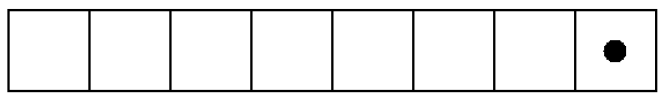
\includegraphics[height=1.5cm]{adventure1}
\end{center}

\end{problem}


\begin{problem}\label{prob:base1.5}
Poindexter decides to play with a system that follows
the rule $2\leftarrow 3$.
\begin{enumerate}[(a)]
\item
Describe what this rule does when there are three dots in the right-most box.
\item
Draw diagrams or use buttons or pennies to find the $2\leftarrow 3$ codes for the
following numbers:
\[
1, 2, 3, 4, 5, 6, 7, 8, 9, 10, 11, 12, 13, 14, 15, 16, 17, 18, 19, 20, 24, 27, 30, 33, 36, \text{ and }
39
\]
Can you find (and \emph{explain}) any patterns?
\end{enumerate}
\end{problem}


\begin{problem}
Repeat problem \ref{prob:base1.5} for your own rule. Choose two numbers $a$ and $b$ and figure
out what the code is for your $a\leftarrow b$ system for each of the numbers above.
\end{problem}

\end{document}


  
